\documentclass[11pt]{article}
\usepackage{fullpage}
\usepackage{hyperref}
\usepackage{listings}
\usepackage{graphicx}
\usepackage[toc,page]{appendix}
\graphicspath{ {figs/} }

%\usepackage{doublespace}
\begin{document}
\title{Weekly Report - Decomposing Ethash(Shared Memory Implementation)}
\author{MSc Project \\
Runchao Han \\
}
\maketitle

%\begin{figure}[h]
%    \centering
%    \includegraphics[width=0.8\textwidth]{nvp.eps}
%    \caption{Importing the Ethminer to Nvidia Visual Profiler}
%    \label{fig:nvp}
%\end{figure}

%TODO references
\section{Progress of the Last Week}

\begin{enumerate}
\item Decomposed Ethash (Shared Memory Implementation) with the help of a sequence diagram
\item Read paper about optimising CUDA programs
\end{enumerate}

\section{Decomposing Ethash}

The Ethash has two CUDA implementations, both of which have been commented in detail:

\begin{itemize}
\item dagger\_shared.cuh\footnote{\url{https://github.com/SebastianElvis/ethminer/blob/master/libethash-cuda/dagger_shared.cuh}}
\item dagger\_shuffled.cuh (CUDA $\geq$ 9.0)\footnote{\url{https://github.com/SebastianElvis/ethminer/blob/master/libethash-cuda/dagger_shuffled.cuh}}
\end{itemize}

Where the shuffled version is more efficient than the shared memory version.

Ethash can be described as shown in Fig.~\ref{fig:ethash}, which starts from hashing the header and a random nonce, then mixes it with random bits in the DAG(approximately 1G) for 64 times, where accessing DAG is the performance bottleneck.



The meaning of every line of the code is commented in the Github project above. At present, the shared memory implementation has been totally figured out. The next step is to improve its performance.

\section{How to Optimise a CUDA Program}

The shared memory version has several $\_\_syncthreads()$, regarded as barriers. Obviously, this program is not well optimised(The shuffled version has not been well analysed by me yet).

A highly cited paper from UIUC and Nvidia\cite{ryoo2008optimization} illustrates some principles of optimising a CUDA program:

\begin{itemize}
\item Leverage zero-overhead thread scheduling to hide memory latency
\item Optimize use of on-chip memory to reduce bandwidth usage and redundant execution
\item Group threads to avoid SIMD penalties and memory port/bank conflict
\item Threads within a thread block can communicate via synchro- nization, but there is no built-in global communication mechanism for all threads
\end{itemize}

This week the target is to optimise the Ethash shared memory version according to this paper.

%
% This section is used to list the following week's plan
% Use the \item construct to list each item.  Try to keep the
% Descriptions for each down to one or two sentences
%
\section{Next Week's Plan}
\begin{enumerate}
\item Attempt to optimise Ethash shared memory version
\item Figure out Ethash shuffled version
\item Examine CryptoNight algorithm
\item Import CryptoNight miner to Eclipse
\end{enumerate}

\bibliographystyle{plain}
\bibliography{references.bib}

\begin{appendices}

\begin{figure}[h]
    \centering
    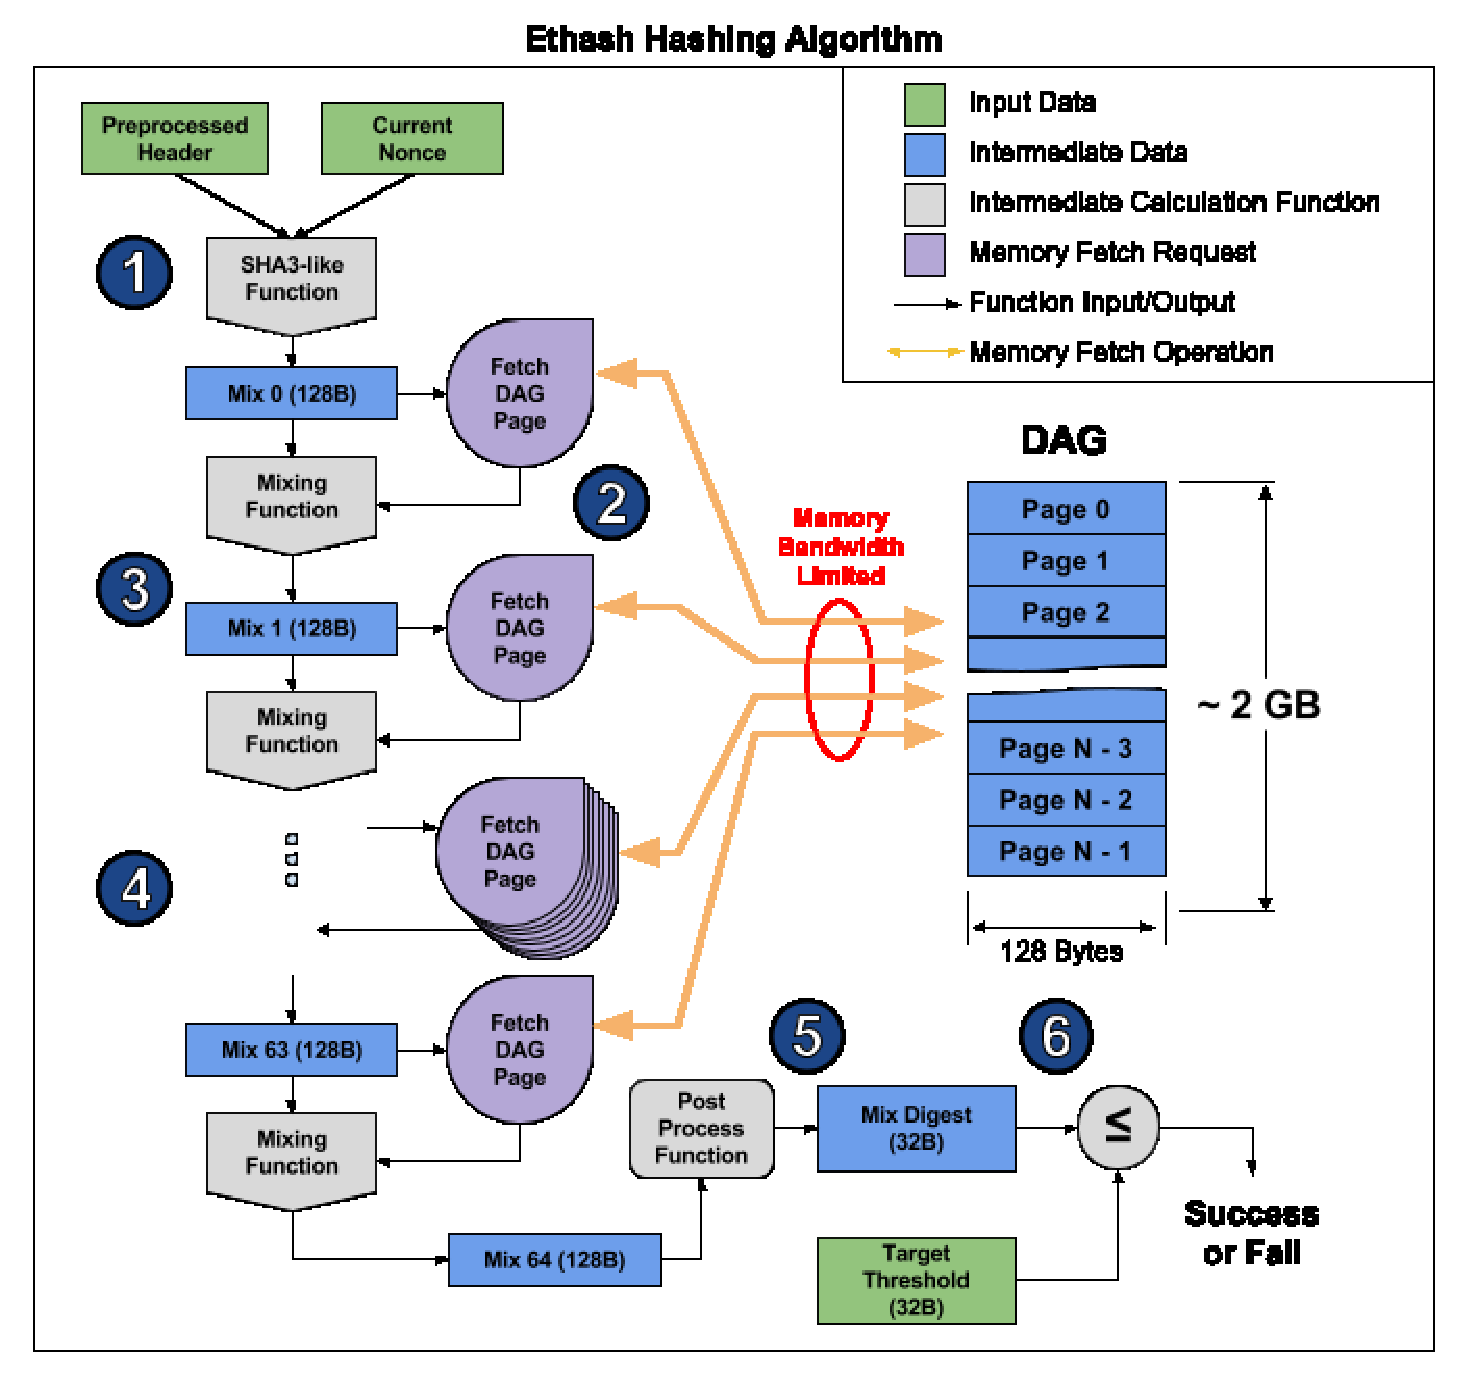
\includegraphics[width=\textwidth]{ethash.eps}
    \caption{The process of Ethash mining algorithm}
    \label{fig:ethash}
\end{figure}

\end{appendices}

\end{document}
